% !TEX root = ../Thesis.tex
%%
%%  Hochschule für Technik und Wirtschaft Berlin --  Abschlussarbeit
%%
%% Kapitel 2 - Grundlagen
%%
%%


\chapter{Grundlagen} \label{Grundlagen}

%Die Aufgabenstellung umfasst die Implementierung eines Smart Objects. Dieses Kapitel behandelt die Grundlagen von Smart Objects. Dabei werden zuerst zentrale Begriffe beschrieben, die in dieser Arbeit verwendet werden. Teilweise handelt es sich um englische Begriffe, weil diese auch in der deutschen Literatur gebräuchlicher sind.

In diesem Kapitel wird nach anfänglichen Begriffserklärungen der schematische Hardwareaufbau eines Smart Objects erläutert. Es wird ein Überblick über verschiedene Technologien, die im Zusammenhang mit der Aufgabenstellung verwendet werden können, gegeben. Diese Technologien werden hier kurz angesprochen und einsortiert. Technische Details werden, soweit notwendig, in späteren Kapiteln erörtert.

%Verschiedene Übertragungstechniken und Kommunikationstechnologien, die im Zusammenhang mit Smart Objects und Sensornetzen eingesetzt werden, werden vorgestellt. Es wird ein Überblick über verschiedene Technologien, die im Zusammenhang mit Smart Objects und drahtlosen Sensornetzen verwendet werden, gegeben. Diese Technologien werden hier kurz angesprochen und einsortiert. Technische Details werden, soweit notwendig, in späteren Kapiteln erörtert.

Um darzustellen, wie ein Benutzer auf die zu implementierende Lösung zugreifen kann, werden verschiedene Applikationen vorgestellt. Außerdem werden verschiedene Betriebssysteme vorgestellt, die für eine Softwareimplementierung in Frage kommen.

Zum Abschluss dieses Kapitels werden technische und nicht-technische Herausforderungen angesprochen. 
\footnote{Dieses Kapitel behandelt verschiedene Technologien, die von Smart Objects benutzt werden könnten. Zuerst werden allgemein die Anforderungen und Herausforderungen hervorgehoben und später die verschiedenen Technologien unter diesem Aspekt erläutert. Die Einteilung der Technologien ist an das TCP/IP-Modell angelehnt.}
%{\color{red}{in Bezug zur Arbeit oder in Anwendung in Smart Objects. Nicht nur einfach Grundlagen.
%und: einteilung in TCP/IP-Modell teilweise schwierig, weil manche Standards alle Layer umfassen. Vielleicht einordnen in Smart Objects %Hardware, Kommunikationsmedien, Kommunikationstechnologien, Benutzerschnittstellen, Smart Objects Softwareumgebungen}}

\section{Begriffserklärungen}

Um die später vorgestellten Übertragungstechniken und Kommunikationstechnologien besser einordnen zu können, wird zu Beginn auf das OSI-7-Schichtenmodell \index{OSI-Modell}eingegangen.

Außerdem werden weitere Begriffe erläutert, die helfen sollen, die zu implementierende Lösung einzugruppieren. Teilweise handelt es sich um englische Begriffe, weil diese auch in der deutschen Literatur gebräuchlicher sind.

%Smart Objects haben sehr viele Gemeinsamkeiten mit zwei anderen Forschungsfeldern. Eingebettete Systeme verwenden oft ähnliche Hardware, in drahtlosen Sensornetzen werden häufig ähnliche Kommunikationstechnologien eingesetzt. Beide Begriffe werden kurz vorgestellt, um darauf folgend den Begriff Smart Object genauer zu erläutern und zu beschreiben, wie sich ein Smart Object von den beiden anderen Begriffen unterscheidet.

%Das Internet-of-Things ist ein Begriff, der immer häufiger in der Literatur verwendet wird. Er beschreibt eine Vision, wie sich das Internet in Zukunft entwickeln kann. Dies hat einen großen Einfluß auf die Entwicklung von Smart Objects.

\subsection{OSI-7-Schichtenmodell}

Das OSI-7-Schichtenmodell wird als bekannt vorausgesetzt. Weil es aber verschiedene Interpretationen und Namensgebungen gibt, werden in der Tabelle \ref{tab:OSI-7-Schichtenmodell} Begriffe zugeordnet, wie sie in dieser Arbeit verwendet werden. Es werden die deutschen und englischen Begriffe für die sieben Schichten aufgelistet. Zusätzlich wird die Einordnung nach dem TCP/IP-Modell \citep{RFC1122} gezeigt und es werden für jede Schicht Beispielprotokolle genannt.

\begin{table}[htbp]
\caption{OSI-7-Schichtenmodell}
\resizebox{\textwidth}{!}{
\begin{tabular}{|c|c|c|c|c|}\hline
  \multicolumn{3}{|c|}{\textbf{Schicht}} & \textbf{Beispielprotokoll} & \textbf{TCP/IP-Modell} \\ \hline
  7 & Anwendungsschicht & Application Layer & \multirow{3}{*}{HTTP, FTP, SNMP} & \multirow{3}{*}{Application Layer} \\ \cline{1-3}
  6 & Darstellungsschicht & Presentation Layer & & \\ \cline{1-3}
  5 & Sitzungsschicht & Session Layer & & \\ \hline
  4 & Transportschicht & Transport Layer & TCP, UDP & Transport Layer \\ \hline
  3 & Vermittlungsschicht & Networking Layer & IPv4, IPv6, ICMP & Internet Layer \\ \hline
  2 & Sicherungsschicht & Data Link Layer & \multirow{2}{*}{Ethernet, WLAN, ISDN} & \multirow{2}{*}{Link Layer} \\ \cline{1-3}
  1 & Physikalische Schicht & Physical Layer & & \\ \hline
\end{tabular}
}
\label{tab:OSI-7-Schichtenmodell}
\end{table}

Das OSI-7-Schichtenmodell wird in dieser Arbeit verwendet, um Übertragungstechniken und Kommunikationstechnologien einordnen zu können.

\subsection{Eingebettete Systeme}

Eingebettete Systeme \index{Embedded System} -- oft wird auch der englische Begriff embedded systems verwendet -- sind kleine Computer, die Teilaufgaben in einem größeren technischen Kontext übernehmen. Sie bestehen häufig aus Mikrocontrollern oder digitalen Signalprozessoren und sind dafür ausgelegt eine bestimmte Funktion, oder auch mehrere bestimmte Funktionen, zu übernehmen. Im Gegensatz zu herkömmlichen Computern ist es nicht möglich, die Funktion eines eingebetteten Systems zu ändern \cite{Heath:EmbeddedSystemsDesign}.

\subsection{Drahtlose Sensornetze}

\begin{figure}[htbp]
	\centering
	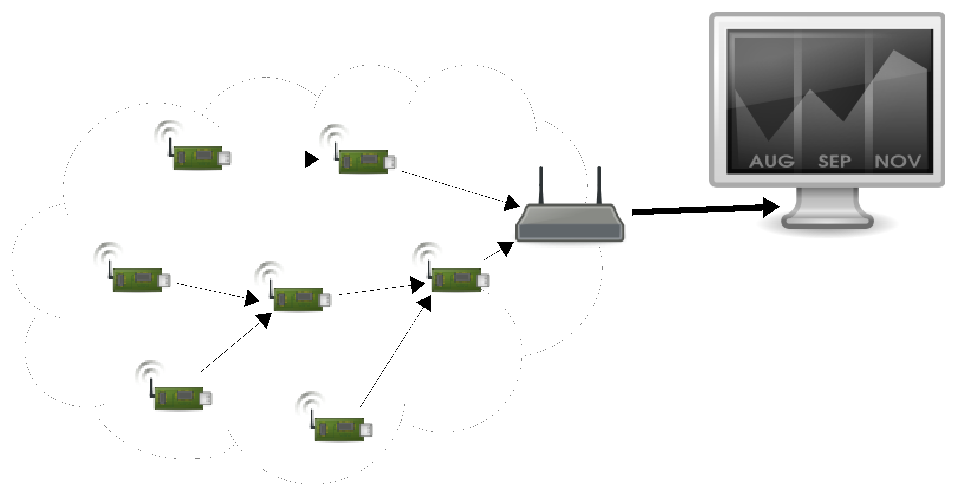
\includegraphics[width=12cm]{wireless_sensor_network}
	\caption{Aufbau eines drahtlosen Sensornetzwerkes}
	\label{fig:wsn}
\end{figure}

Bei drahtlosen Sensornetzen, international auch Wireless Sensor Networks (WSN) genannt, handelt es sich um Netzwerke aus kleinen Sensoren, die ihre Messergebnisse zu einer zentralen Station senden. Die Sensoren helfen dabei einander, die Informationen weiterzureichen (siehe Abbildung \ref{fig:wsn}). So ein drahtloses Sensornetz kann zum Beispiel in einem Gebäude Temperatur- und Luftfeuchtigkeitswerte an eine zentrale Station liefern, die dann die Klimaanlage entsprechend ansteuert. Eine komplette Verkabelung jedes einzelnen Sensors kann dabei je nach Anzahl sehr aufwendig und kostspielig sein. Wenn die Sensoren dazu noch mobil sein sollen, empfiehlt sich eine drahtlose Kommunikation.

Ein Sensor in einem drahtlosen Sensornetz ist ausgestattet mit einer Kommunikationseinheit, die sich selbstständig innerhalb des Netzes konfiguriert und darüber die eingelesenen Messgrößen zu einer zentralen Stelle transportiert.

%%Ein Sensor ist dabei ein typisches Smart Object. Es 
%% Das Steuergerät soll dabei möglichst klein sein, damit es in einem Steckdosengehäuse Platz finden kann. 
%% Der Fernzugriff soll mithilfe des Protokolls IPv6 erfolgen, um zukunftssicher auf die Infrastruktur des Internet verwenden zu können. 

\subsection{Smart Objects}\label{Smart Objects}

Diese Definition von Smart Objects \index{Smart Object} beruht auf \textcite{vasseur10interconnecting}. Dabei handelt es sich um kleine Objekte, die mit folgenden Einheiten ausgestattet sind:

\begin{itemize}
	\itemsep 0pt
	\item eine Form von Sensor und/oder Aktor
	\item ein kleiner Mikrocontroller
	\item eine Kommunikationseinheit
	\item eine Energieversorgung
\end{itemize}

Ein Sensor und/oder Aktor wird benötigt, um mit der Umwelt interagieren zu können. Ein Sensor kann bestimmte Messgrößen erfassen, die dann verarbeitet werden können. Ein Aktor ist das Gegenstück zu einem Sensor. Über ihn kann aktiv die Umwelt beeinflusst werden. Die Kommunikationseinheit befähigt das Smart Object über ein Netzwerk kommunizieren zu können. Es ist dabei möglich mit anderen Smart Objects zu kommunizieren als auch mit weit entfernten Geräten, im Falle des Internets weltweit. Ein kleiner Mikrocontroller übernimmt die Informationsverarbeitung. Dieser nimmt Daten von Sensoren entgegen bzw. steuert den Aktor. Die Kommunikation wird ebenso von ihm geregelt, von einem Sensor gemessene Werte können über das Netzwerk weitergegeben werden. Der Mikrocontroller kann als Kern des Smart Object angesehen werden. Die Energieversorgung ist notwendig, um alle Einheiten ausreichend mit elektrischer Energie zu versorgen.

Alle diese technischen Eigenschaften machen ein Objekt aber noch nicht zu einem Smart Object. Erst die Anwendung und sein Verhalten machen aus einem Objekt mit den obigen Eigenschaften ein Smart Object. Allerdings ist es sehr schwierig, dieses Verhalten zu definieren. Die Anwendungen sind sehr unterschiedlich und es ist völlig unbekannt, wie Smart Objects in der Zukunft eingesetzt werden. Gemeinsam ist allen Anwendungen allerdings, dass Smart Objects mit der physikalischen Umwelt interagieren und über ein Netzwerk kommunizieren. Dieses Verhalten und die obigen technischen Eigenschaften machen ein Smart Object aus.

Von der Kommunikationstechnologie her ähnelt ein Smart Object einem Sensor in einem Sensornetz. Allerdings ist im Gegensatz zu einem Sensornetz ein Netz aus Smart Objects nicht allein auf die Datenübermittlung fokussiert. Bei einem Sensornetz ist der Datenfluss immer vom Sensor ins Netzwerk, wohingegen der Datenfluss bei einem Smart Object bidirektional ist. Der Fokus liegt dabei auf eine Vielzahl von Funktionen insbesondere der Steuerung und Überwachung \citep[Seite 12]{vasseur10interconnecting}. Es ist also die Anwendung, die ein Gerät zu einem Smart Object macht. Aber Entwicklungen, hauptsächlich in der Energieversorgung und Kommunikationstechnik, kommen beiden Forschungsgebieten zugute.


\subsection{Internet-of-Things}

\begin{figure}[htbp]
	\centering
	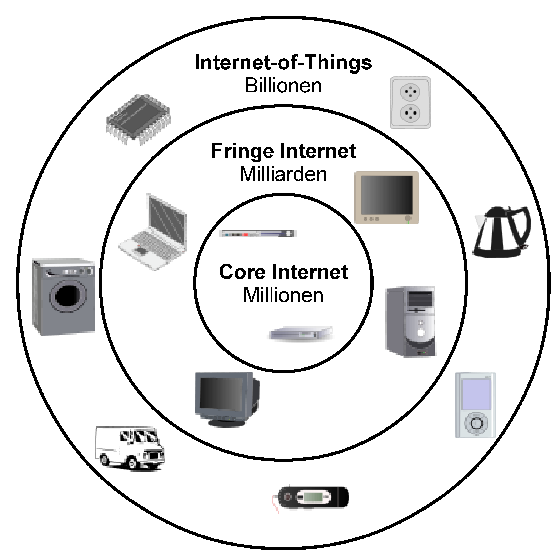
\includegraphics{internet_of_things}
	\caption{Die Internet-of-Things Vision \cite[Figure 1.2]{Bormann:6LoWPAN}}
	\label{fig:internet_of_things}
\end{figure}

Das Internet-of-Things, auch Internet der Dinge genannt, ist eine Vision, wie sich das Internet in Zukunft entwickeln kann. Es soll aus der Vernetzung vieler Kleinstgeräte -- auch oder vielleicht hauptsächlich Smart Objects -- bestehen. \textcite{Bormann:6LoWPAN} betrachten das Internet-of-Things als eine weitere Schale des Internets (Abbildung \ref{fig:internet_of_things}), die gerade anfängt sich heraus zu bilden. Der Kern des Internets (Core Internet) besteht heute aus vielen Routern und Servern, die zusammen Millionen von Teilnehmern ausmachen. Um diesen Kern herum liegt das sogenannte Fringe Internet, was beispielsweise aus privaten Rechnern oder Laptops besteht, aber auch aus lokalen Netzwerken, die zum Internet verbunden werden. Die Teilnehmer des Fringe Internet gehen in die Milliarden. Um dieses Fringe Internet herum beginnt sich eine weitere Schale zu bilden, das sogenannte Internet-of-Things. Auf lange Sicht kann hier mit Billionen von Teilnehmern gerechnet werden. Hauptsächlich bestehen diese Teilnehmer aus IP-fähigen eingebetteten Systemen (embedded systems). Eine so große Zahl an Teilnehmern kann nur mithilfe des Internet Protokolls der Version 6 ans Internet angeschlossen werden, da das bisherige Internet Protokoll der Version 4 keine freien Adressräume mehr zur Verfügung hat.

\section{Theoretische Grundlagen}
\ldots
\section{Kommunikationstechnologien}
\ldots
\section{Betriebssysteme für SmartObjects}
\ldots
\section{Zusammenfassung/Bewertung}
\ldots